\chapter{Training and technologies}
\label{chap:ch5}

\section{Training}
\label{sec:ch5sec1}

\subsection{Dataset}
\label{subsec:ch5sec1subsec1}

The dataset consists of chess matches played at grandmaster level downloaded in PGN format from the website chessabc.com \cite{chessabc}.

A PGN (portable game notation) file contains multiple chess matches. Each match has several headers (name of player with white pieces, name of player with black pieces, event it was played at, date it was played on, result, elo of players etc.), an empty line, and then the "movetext section". The matches in a PGN file are separated by two empty lines. Following is a sample PGN match:
\begin{figure}[h]
    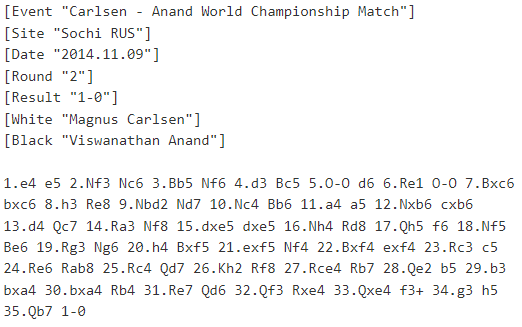
\includegraphics[width=0.8\textwidth]{figures/carlsen-anand-match.png}
\end{figure}

The movetext section contains the chess moves, move numbers, optional annotations and a concluding game termination marker (the result of the match). The result can be "1-0" (white won), "0-1" (black won) or "1/2-1/2" (draw). The moves are written in SAN (standard algebraic notation). SAN identifies each square on the board as a combination of file (a-h) and rank (1-8) (see fig. \ref{fig:boardSquares}).

\begin{figure}[h]
    \centering
    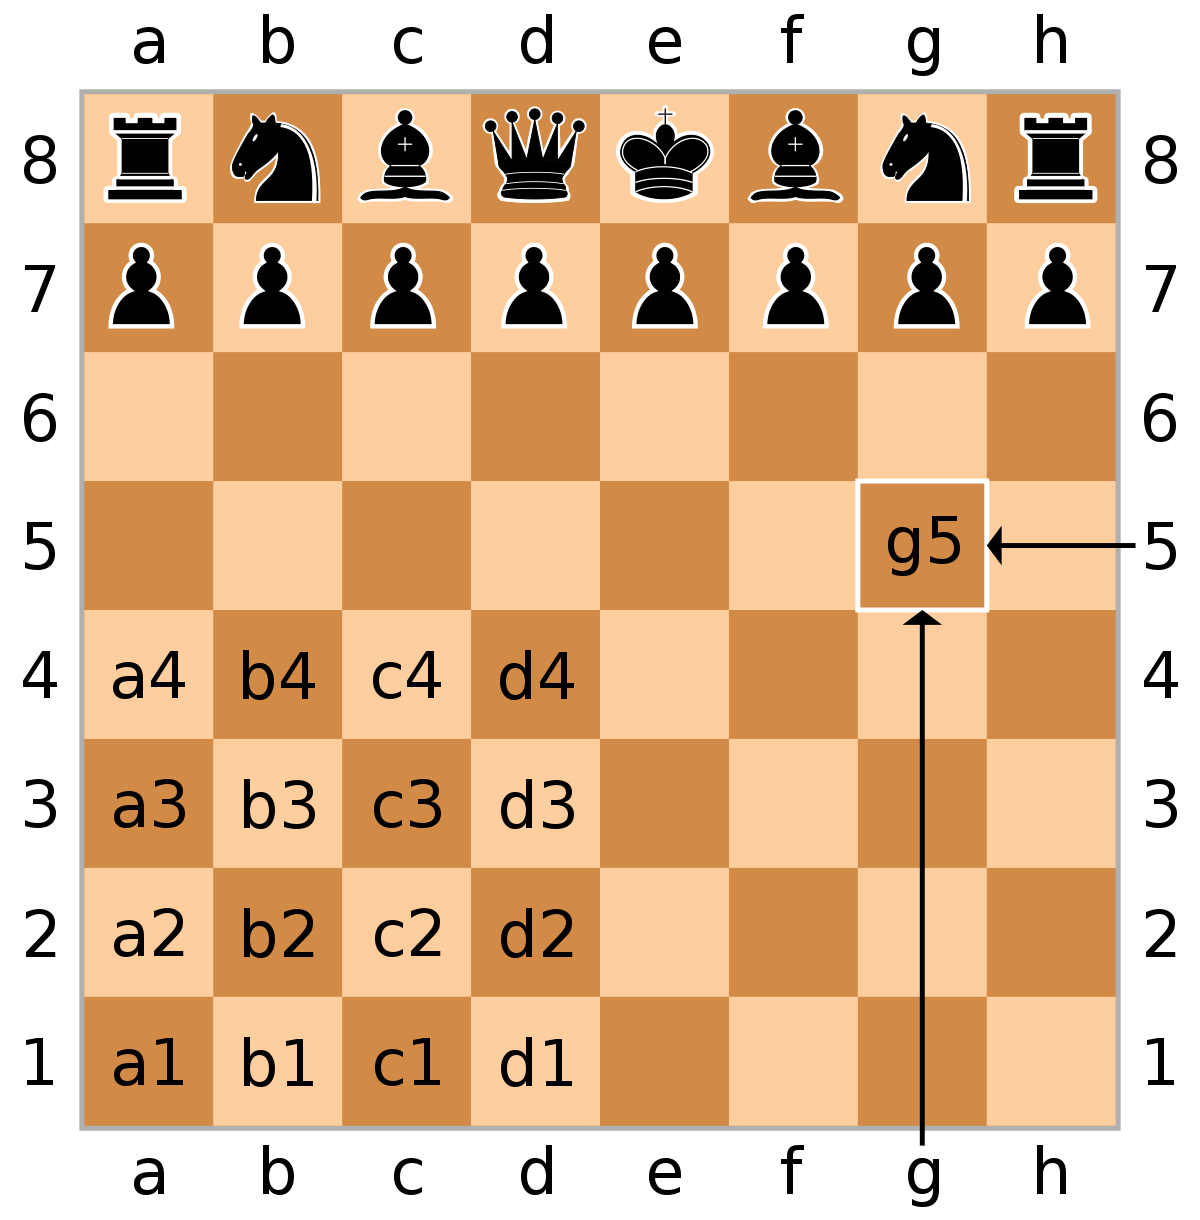
\includegraphics[width=0.4\textwidth]{figures/board-squares.png}
    \caption{Board squares}
    \label{fig:boardSquares}
\end{figure}

Each piece can be identified by a letter (K - king, Q - queen, R - rook, B - bishop, N - knight, P - pawn). Simple SAN moves contain only the destination square, and the letter of piece that moves, if the piece is not a pawn (for example, pawn to c6 is written simply as c6, while knight to c6 is written as Nc6). There are additional rules for moves \cite{edwards1994standard}:
\begin{itemize}
    \item Moves that capture a piece contain the 'x' character right before the destination square (ex: Bxb4)
    \item Castling kingside is written as 'O-O', while queenside castling is written as 'O-O-O'
    \item Moves of pawns to the last rank (promotion moves) contain the equal sign ('=') right after the destination square, followed by the letter of the piece that the pawn promotes to (ex: e8=Q)
    \item If there are multiple pieces of the same type that can move to the destination square, the file of the originating square is added right after the piece (ex: Nbc6); if this does not solve the ambiguation, the rank of the originating square is added instead (ex: N8c6), and if neither of these works, both the file and the rank are added (ex: Nb8c6)
    \item If the move checks the opponent's king, a plus sign ('+') is added at the end of the move (ex: Qe7+); if the move checkmates the opponent's king, the octothorpe sign ('\#') is added instead (ex: Qe7\#)
\end{itemize}

I computed the positions that occured in the matches in the dataset, and the value I assigned to each position is the mean of the results of the matches in which the position appeared. For example: if position A appeared in 10 matches, and 4 of the matches ended in a win for white, 2 in a win for black, and the other 4 were draws, the value assigned to the position is: \[((4*1)+(4*0)+(2*-1))/10=0.2\] (a win for white is assigned 1, a win for black is assigned -1, and a draw is 0).

% 100 epoci, batch-size 64
% Number of positions: 8493798, number of distinct positions: 5586478

\subsection{Layers}
\label{subsec:ch5sec1subsec2}

\section{Technologies}
\label{sec:ch5sec2}

% Details of the programming languages, libraries, and tools used

\subsection{Chess game}
\label{subsec:ch5sec2subsec1}

% Description of tools used in building the chess game - Unity, C\#

\subsection{Chess engine}
\label{subsec:ch5sec2subsec2}

% Description of tools used in building the chess engine - C\#, keras